\section{Problem 1}
\subsection{Discussion}
\noindent \textbf{Disclamer} For Random Query attacks, the benchmarks I ran stop short of a couple of combinations of very large $n$ and $m$. The least squares optimization becomes extremely slow for those cases. My Computer has a lot of memory and several cores, if I could parallelize or otherwise optimize that step, I would be able to run the experiments much quicker. In all cases, the experiments did not fail for these combinations, they just took a long time to finish a few runs, so I stopped them as to not waste time. \\

\noindent \textbf{Plots vs Theory} The plots seem to confirm the theory. If we treat $\alpha = \sigma$, then we can see that the accuracy of the attack is severely low for $\alpha$ close to half, the noise is very big (as big as rounding) to the extent that we are left guessing randomly, hence the accuracy is close to 0.5. \\

\noindent As $\alpha$ becomes smaller, the accuracy increases near the theoretical limit of $4 \sigma^2 n$. I plotted the accuracy vs the theoretical limit for each $n$ attempted in figure~\ref{fig:hadamard-theory}. I only show the figure for $N=512$ for brevity, but similar figures for all $n$ are available (and in higher quality) at: \\
\href{https://github.com/KinanBab/PrivacyInMachineLearning/tree/master/Homework1/1-Hadmard-Random-Attacks/plots}{https://github.com/KinanBab/PrivacyInMachineLearning/tree/master/Homework1/1-Hadmard-Random-Attacks/plots} \\

\noindent \textbf{Comparing the two attacks:} The nice thing about the Hadamard load (or the bad thing, depending on how you look at it), is that you can reconstruct with high accuracy with $n$ queries. The runtime for it is also fast, since the attack does not involve optimizations or matrix inversions. The random query attack needs $m$ to be much larger than $n$ to become effective, as shown in the plots, which means the number of queries is large, and the run-time needed to carry out the attack is larger (larger dimensions and more expensive operations).

\noindent \textbf{Choice of $m$:} Random Query attacks perform poorly when $m$ is small compared to $n$. However, if sigma is very small (close to $\frac{1}{\sqrt(32n)}$), the accuracy is improved even for small $m$.

\noindent \textbf{Average Deviation:} In All the experiments (both hadamard and random querys), the average deviation is small (< 0.02). It decreases very quickly in $n$ and $m$, but seems independent from $\sigma$.

\begin{figure}
    \centering
    \begin{subfigure}[b]{0.5\textwidth}
        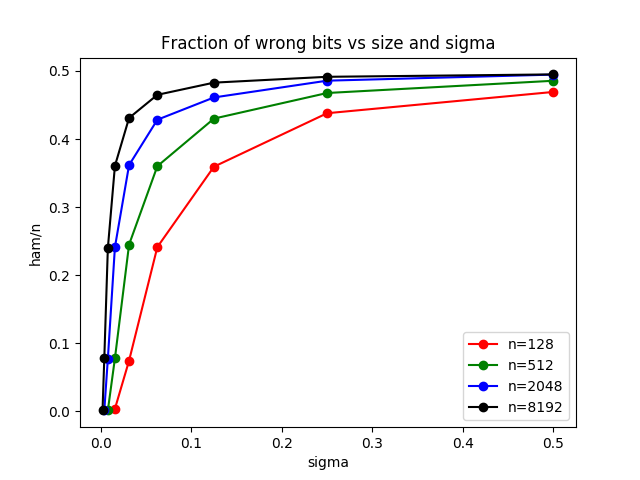
\includegraphics[width=\textwidth]{hadmard/Hadamard-all.png}
        \caption{Overall Accuracy for All $n$}
        \label{fig:hadamard-all}
    \end{subfigure}
    \begin{subfigure}[b]{\textwidth}
        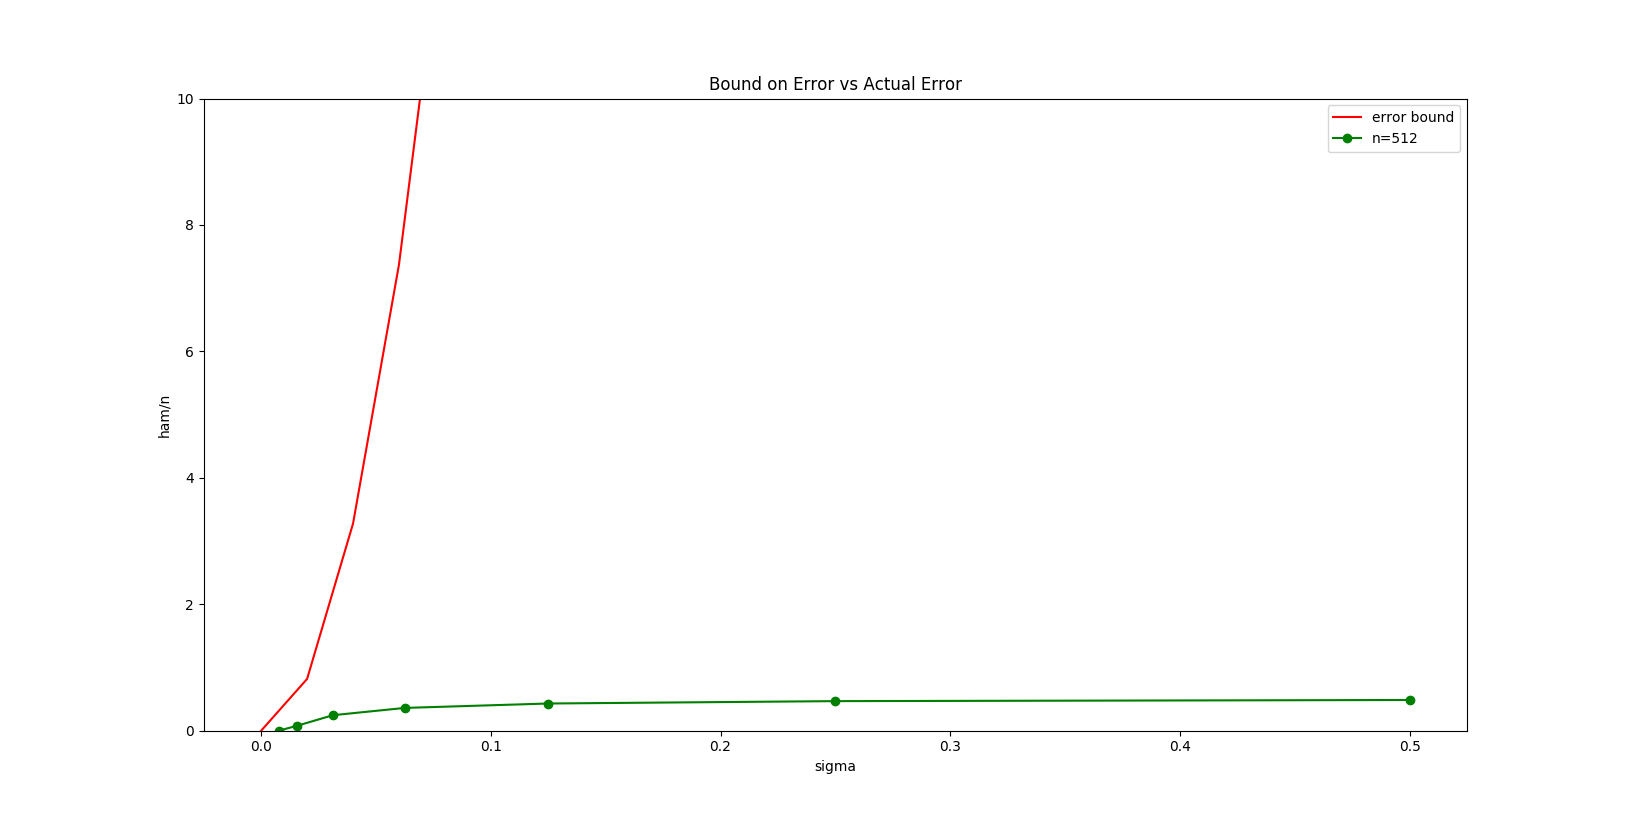
\includegraphics[width=\textwidth]{hadmard/Hadamard-N512.png}
        \caption{Accuracy for $n=2048$ Compared To Theoretical Bound}
        \label{fig:hadamard-theory}
    \end{subfigure}
    \caption{Plots for Hadamard Attack}\label{fig:hadamards}
\end{figure}

\begin{figure}
    \centering
    \begin{subfigure}[b]{0.49\textwidth}
        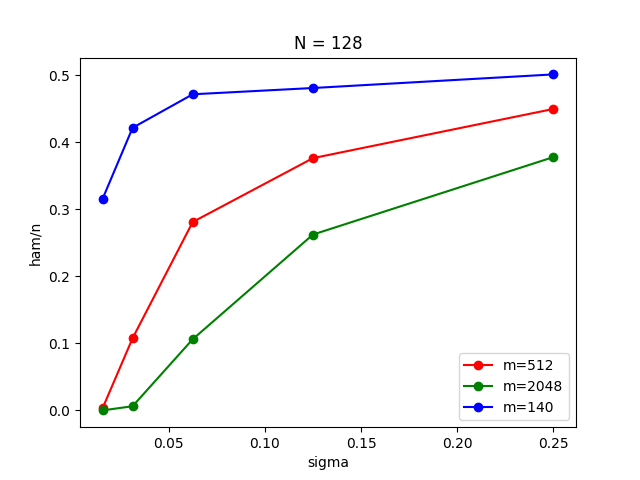
\includegraphics[width=\textwidth]{random/Random-N128.png}
        \caption{Accuracy for $n=128$ and several $m$}
    \end{subfigure}
    \begin{subfigure}[b]{0.49\textwidth}
        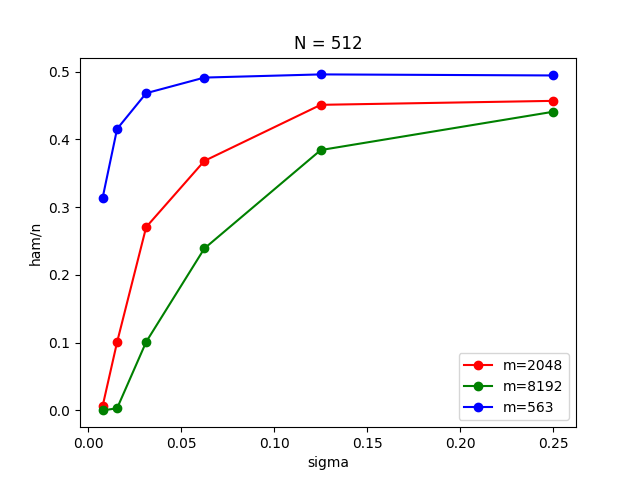
\includegraphics[width=\textwidth]{random/Random-N512.png}
        \caption{Accuracy for $n=512$ and several $m$}
    \end{subfigure}
    \begin{subfigure}[b]{0.49\textwidth}
        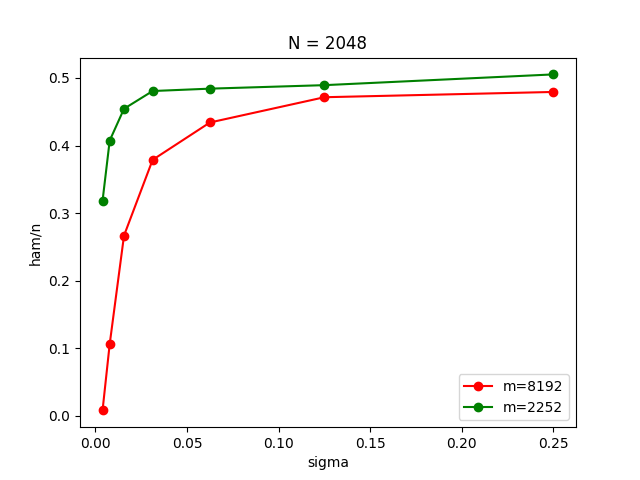
\includegraphics[width=\textwidth]{random/Random-N2048.png}
        \caption{Accuracy for $n=2048$ and several $m$}
    \end{subfigure}
    \begin{subfigure}[b]{0.49\textwidth}
        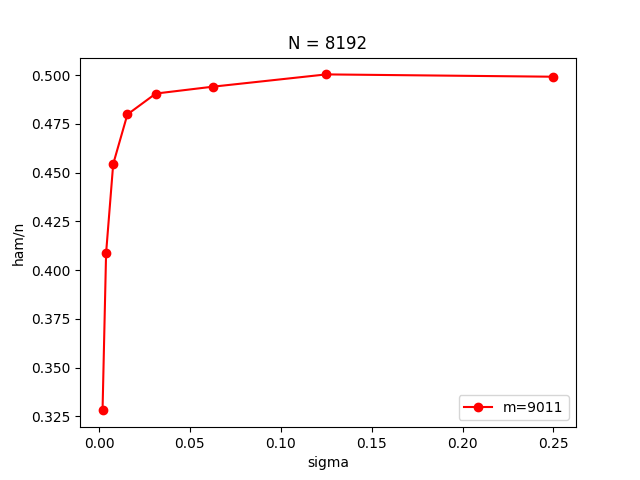
\includegraphics[width=\textwidth]{random/Random-N8192.png}
        \caption{Accuracy for $n=8192$ and $m=1.1n$}
    \end{subfigure}
    \caption{Plots for Random Query Attack}\label{fig:random}
\end{figure}